% Model Cards pipeline figure.
% Adapted from the shipped Auto-BenchmarkCards Figure 1 visual grammar.
% The figure ends at a generated candidate. Human release review is not shown
% because it has not yet been completed for the examples in this repository.
\documentclass[tikz,border=3pt]{standalone}

\usepackage{newtxtext,newtxmath}
\usepackage{xcolor}
\usepackage{tikz}
\usetikzlibrary{arrows.meta,calc}

\definecolor{Ink}{HTML}{1A1A1A}
\definecolor{Ink60}{HTML}{6E6E6E}
\definecolor{Rule}{HTML}{D9D9D9}
\definecolor{Blue700}{HTML}{1F4E9C}

% A single exact checkpoint selected from related model snapshots.
\newcommand{\icnIdent}[2]{%
\begin{scope}[shift={#1}]
\begin{scope}[x={#2},y={#2},shift={(1.74,0.29)},line join=round,line cap=butt]
  \foreach \ang in {16,8}{%
    \begin{scope}[rotate around={\ang:(-3.9,-4.8)}]
      \fill[white] (-3.9,-4.8) rectangle (2.5,2.8);
      \draw[Ink,line width=1.1pt,rounded corners=0.5mm]
            (-3.9,-4.8) rectangle (2.5,2.8);
    \end{scope}}
  \fill[Ink,rounded corners=0.5mm] (-3.9,-4.8) rectangle (2.5,2.8);
  \fill[white] (-3.0,0.9) rectangle (1.6,1.9);
  \foreach \yy in {-0.5,-1.7}{
    \draw[white,line width=0.9pt] (-3.0,\yy)--(1.6,\yy);}
  \draw[white,line width=0.9pt] (-3.0,-2.9)--(-0.8,-2.9);
\end{scope}\end{scope}}

% Document, structured metadata, developer code, and linked public records.
\newcommand{\icnSources}[2]{%
\begin{scope}[shift={#1}]
\begin{scope}[x={#2},y={#2},shift={(-0.01,0.05)},line join=round,line cap=butt]
  \foreach \p in {(-4.9,3.5),(-4.9,-3.5),(4.9,3.5),(4.9,-3.5)}{
    \draw[Ink,line width=1.2pt] (0,0)--\p;}
  \fill[Ink] (-6.35,2.05)--(-6.35,4.95)--(-4.35,4.95)--
             (-3.45,4.05)--(-3.45,2.05)--cycle;
  \fill[white] (-4.35,4.95)--(-4.35,4.05)--(-3.45,4.05)--cycle;
  \foreach \yy in {3.35,2.75}{
    \draw[white,line width=0.7pt] (-5.65,\yy)--(-4.15,\yy);}
  \fill[Ink] (-6.35,-4.5) rectangle (-3.45,-2.5);
  \fill[Ink] (-4.9,-2.5) ellipse (1.45 and 0.55);
  \fill[Ink] (-4.9,-4.5) ellipse (1.45 and 0.55);
  \foreach \yy in {-3.2,-3.95}{
    \draw[white,line width=0.7pt] (-6.35,\yy) arc (180:360:1.45 and 0.5);}
  \fill[Ink,rounded corners=0.55mm] (3.45,2.05) rectangle (6.35,4.95);
  \draw[white,line width=0.85pt,line cap=round,line join=round]
        (4.65,4.35)--(4.05,3.5)--(4.65,2.65);
  \draw[white,line width=0.85pt,line cap=round,line join=round]
        (5.35,4.35)--(5.95,3.5)--(5.35,2.65);
  \fill[Ink] (4.9,-3.5) circle (1.45);
  \draw[white,line width=0.75pt] (4.9,-3.5) ellipse (0.6 and 1.45);
  \draw[white,line width=0.75pt] (3.55,-3.5)--(6.25,-3.5);
  \fill[white] (0,0) circle (2.25);
  \fill[Ink] (0,0) circle (2.0);
\end{scope}\end{scope}}

% Candidate claims enter; only checkpoint-scoped, verified evidence is bound.
\newcommand{\icnBind}[2]{%
\begin{scope}[shift={#1}]
\begin{scope}[x={#2},y={#2},shift={(-1.18,0.45)},line join=round,line cap=butt]
  \foreach \xx in {-2.6,0,2.6}{
    \fill[Ink,rounded corners=0.3mm] (\xx-1.15,3.4) rectangle (\xx+1.15,4.6);}
  \begin{scope}[rotate around={-46:(5.9,1.4)}]
    \fill[white,rounded corners=0.3mm] (4.75,0.8) rectangle (7.05,2.0);
    \draw[Ink,line width=1.1pt,rounded corners=0.3mm]
          (4.75,0.8) rectangle (7.05,2.0);
  \end{scope}
  \fill[Ink,even odd rule]
        (-4.8,2.8)--(4.8,2.8)--(1.0,-1.0)--(1.0,-2.3)--
        (-1.0,-2.3)--(-1.0,-1.0)--cycle
        (-3.3,1.75)--(3.3,1.75)--(0.3,-1.3)--(0.3,-2.3)--
        (-0.3,-2.3)--(-0.3,-1.3)--cycle;
  \fill[Ink,rounded corners=0.5mm] (-2.7,-5.5) rectangle (2.7,-2.7);
  \foreach \yy in {-3.5,-4.3}{
    \draw[white,line width=0.85pt] (-1.9,\yy)--(1.9,\yy);}
  \draw[white,line width=0.85pt] (-1.9,-5.1)--(0.2,-5.1);
\end{scope}\end{scope}}

% Bound evidence is composed into schema fields; one row remains visibly empty.
\newcommand{\icnCompose}[2]{%
\begin{scope}[shift={#1}]
\begin{scope}[x={#2},y={#2},shift={(0.2,0.05)},line join=round,line cap=round]
  \foreach \yy in {3.5,0.7,-2.1}{
    \fill[Ink,rounded corners=0.35mm] (-5.8,\yy-0.65) rectangle (-2.2,\yy+0.65);
    \draw[Ink,line width=1.0pt] (-2.2,\yy)--(-0.7,\yy);}
  \fill[Ink,rounded corners=0.55mm] (-0.8,-5.0) rectangle (5.5,5.0);
  \fill[white] (3.5,5.0)--(5.5,3.0)--(3.5,3.0)--cycle;
  \foreach \yy/\xe in {2.0/4.2,0.5/3.1,-2.5/4.2}{
    \draw[white,line width=0.9pt] (0.2,\yy)--(\xe,\yy);}
  \draw[white,line width=0.9pt] (0.2,-1.0)--(1.45,-1.0);
  \draw[white,line width=0.9pt,dash pattern=on 0.8pt off 0.7pt]
        (1.85,-1.0)--(4.2,-1.0);
  \fill[white] (-5.0,3.5) circle (0.20);
  \fill[white] (-5.0,0.7) circle (0.20);
  \fill[white] (-5.0,-2.1) circle (0.20);
\end{scope}\end{scope}}

% Chunky transport arrow copied from the shipped AISI figure geometry.
\newcommand{\barrow}[2]{%
  \filldraw[fill=Blue700,draw=Blue700,line width=1.0pt,line join=round]
    (#1,#2+0.168) -- (#1+0.483,#2+0.168) -- (#1+0.483,#2+0.337)
    -- (#1+0.820,#2) -- (#1+0.483,#2-0.337) -- (#1+0.483,#2-0.168)
    -- (#1,#2-0.168) -- cycle;}

\begin{document}
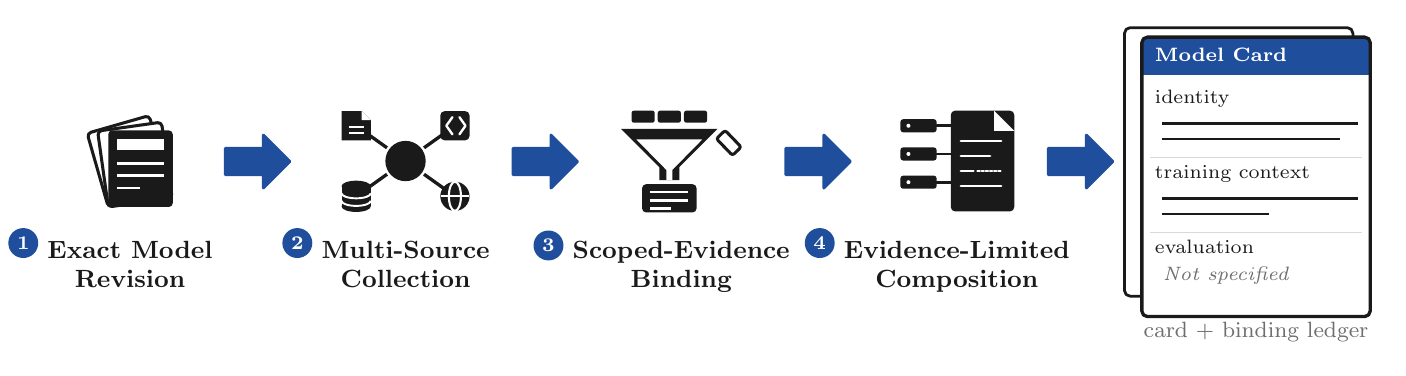
\begin{tikzpicture}[
  x=1cm,y=1cm,line join=round,line cap=butt,font=\scriptsize,
  ttl/.style={font=\small\bfseries,color=Ink,anchor=base,inner sep=0pt},
  lbl/.style={font=\scriptsize,color=Ink,anchor=base west,inner sep=0pt},
  sec/.style={font=\footnotesize,color=Ink60,anchor=base,inner sep=0pt},
  badge/.style={circle,fill=Blue700,text=white,inner sep=0pt,
                minimum size=3.8mm,font=\scriptsize\bfseries}
]
\path[use as bounding box] (0.05,0.90) rectangle (17.20,-3.16);

% Four-stage spine.
\icnIdent{(1.35,-0.80)}{1.28mm}
\icnSources{(4.85,-0.80)}{1.28mm}
\icnBind{(8.35,-0.80)}{1.28mm}
\icnCompose{(11.85,-0.80)}{1.28mm}
\barrow{2.560}{-0.80}
\barrow{6.213}{-0.80}
\barrow{9.678}{-0.80}
\barrow{13.012}{-0.80}

% Stage names.
\node[ttl] (t1) at (1.35,-2.03) {Exact Model};
\node[badge] at ($(t1.west)+(-0.30,0.085)$) {1};
\node[ttl] at (1.35,-2.40) {Revision};

\node[ttl] (t2) at (4.85,-2.03) {Multi-Source};
\node[badge] at ($(t2.west)+(-0.30,0.085)$) {2};
\node[ttl] at (4.85,-2.40) {Collection};

\node[ttl] (t3) at (8.35,-2.03) {Scoped-Evidence};
\node[badge] at ($(t3.west)+(-0.30,0.085)$) {3};
\node[ttl] at (8.35,-2.40) {Binding};

\node[ttl] (t4) at (11.85,-2.03) {Evidence-Limited};
\node[badge] at ($(t4.west)+(-0.30,0.085)$) {4};
\node[ttl] at (11.85,-2.40) {Composition};

% Generated card in front, retained field-level ledger behind it.
\fill[white,rounded corners=2pt] (13.98,-2.51) rectangle (16.88,0.90);
\draw[rounded corners=2pt,draw=Ink,line width=1.0pt]
      (13.98,-2.51) rectangle (16.88,0.90);
\foreach \yy/\xe in {0.46/16.58,0.16/16.18,-0.14/16.58}{
  \draw[Rule,line width=0.8pt] (14.20,\yy)--(\xe,\yy);}

\begin{scope}
\clip[rounded corners=2pt] (14.20,-2.769) rectangle (17.10,0.780);
\fill[Blue700] (14.20,0.300) rectangle (17.10,0.780);
\fill[white] (14.20,-2.769) rectangle (17.10,0.300);
\end{scope}
\draw[rounded corners=2pt,draw=Ink,line width=1.2pt]
      (14.20,-2.769) rectangle (17.10,0.780);
\node[font=\scriptsize\bfseries,text=white,anchor=base west,inner sep=0pt]
      at (14.36,0.475) {Model Card};
\node[lbl] at (14.36,-0.066) {identity};
\foreach \yy/\xe in {-0.318/16.94,-0.513/16.72}{
  \draw[Ink,line width=1.0pt] (14.46,\yy)--(\xe,\yy);}
\draw[Rule,line width=0.4pt] (14.30,-0.746)--(17.00,-0.746);
\node[lbl] at (14.36,-1.020) {training context};
\foreach \yy/\xe in {-1.272/16.94,-1.467/15.82}{
  \draw[Ink,line width=1.0pt] (14.46,\yy)--(\xe,\yy);}
\draw[Rule,line width=0.4pt] (14.30,-1.696)--(17.00,-1.696);
\node[lbl] at (14.36,-1.970) {evaluation};
\node[font=\scriptsize\itshape,color=Ink60,anchor=base west,inner sep=0pt]
      at (14.46,-2.313) {Not specified};
\node[sec] at (15.65,-3.030) {card + binding ledger};

\end{tikzpicture}
\end{document}
